\documentclass[10pt,a4paper]{article}
\usepackage[margin=2.2cm]{geometry}
\usepackage{microtype,graphicx,booktabs,float,xcolor,hyperref,caption,pgfplots,pgfplotstable,enumitem}
\pgfplotsset{compat=1.16}
\hypersetup{colorlinks=true,linkcolor=blue!50!black,citecolor=blue!50!black,urlcolor=blue!50!black}
\setlist{nosep,leftmargin=1.4em}
\captionsetup{font=small,labelfont=bf}
\setlength{\parskip}{3pt}
\usepackage{titlesec}
\titleformat{\section}{\large\bfseries}{\thesection.}{0.5em}{}
\titlespacing*{\section}{0pt}{10pt}{4pt}

\begin{document}
%------------------------------------------------ COVER PAGE
\begin{titlepage}
\centering
\vspace*{1.2cm}
{\large Department of Computer Science and Engineering}\\[0.4cm]
\rule{\textwidth}{0.8pt}\\[0.6cm]
{\Large\bfseries CSE-307: Operating Systems}\\[0.3cm]
{\large Term Paper --- Track 1}\\[1.4cm]
{\LARGE\bfseries Learning-Augmented Page Replacement:\\[0.2cm] Classical Algorithms Meet Adaptive Prediction}\\[0.5cm]
{\large Page Faults on a Student Laptop When the Workload Changes}\\[0.6cm]
\rule{\textwidth}{0.8pt}\\[1.8cm]
\begin{tabular}{r@{\hspace{1em}}l}
\textbf{Course Code:} & CSE-307\\[6pt]
\textbf{Course Name:} & Operating Systems\\[6pt]
\textbf{Student Name:} & Farhan Sadik Tahsin\\[6pt]
\textbf{Student ID:} & 202414072\\[6pt]
\textbf{Level:} & [Level / Term]\\[6pt]
\textbf{Section:} & [Section]\\[6pt]
\textbf{Date:} & 04 October 2026\\
\end{tabular}
\vfill
{\small Code, raw results and figures: \texttt{[your GitHub repository link]}}
\end{titlepage}

%------------------------------------------------ BODY
\begin{center}
{\Large\bfseries Learning-Augmented Page Replacement: Classical Algorithms Meet Adaptive Prediction}\\[4pt]
{\small Farhan Sadik Tahsin \quad ID: 202414072 \quad CSE-307 \quad Track 1}
\end{center}

\section{Problem Framing}
When a page is referenced and every physical frame is full, the operating system must pick a resident page to evict. FIFO and LRU are cheap online policies, while Belady's Optimal policy evicts the page whose next use is farthest in the future. Optimal needs future knowledge, so it is only an offline upper bound~\cite{belady1966,silberschatz}. FIFO and LRU assume the access pattern stays stable, but programs move between phases with different localities~\cite{denning1968}.

The scenario here is deliberately simple. Imagine a student's laptop with very little free memory. For the first half of the session the student works on one assignment, repeatedly switching between a handful of files (code, notes, report). In the second half the assignment is submitted and the student starts browsing, opening many different things in no particular order. The question is: \emph{if a small learned eviction policy is trained while the student is working on the assignment, does it still help after the behaviour changes?}

\section{Implementation and Learned Component}
The simulator (\texttt{src/run\_experiment.py}, pure Python, no external packages) uses 4 frames and 10 pages. FIFO evicts the page loaded earliest, LRU the page with the oldest last reference, and Optimal the resident page whose next reference is farthest away (or never occurs).

The \textbf{learned policy} is a small decision tree (CART-style, Gini impurity, depth 3)~\cite{cart} written from scratch. At every fault with full memory, each resident page is a candidate described by four features known at that moment: \emph{age} (time since loaded), \emph{access frequency}, \emph{recency rank}, and \emph{page id}. The training label is 1 if Belady's Optimal would evict that candidate, else 0. Training uses a separate locality-only trace (seed 2026, 400 references, 192 labelled rows). At run time the policy evicts the candidate with the highest predicted probability of being the Optimal victim, breaking ties by LRU. Future references are never given to the model as features; they are used only to create labels offline.

As an extension, a \textbf{Hybrid} policy runs a shadow LRU cache and, over a sliding window of 40 references, falls back to LRU eviction whenever the shadow LRU has more hits than the hybrid itself. This is a cheap online drift check without retraining.

\section{Experimental Setup}
The evaluation trace has 800 references generated with fixed seed 307 and two 400-reference phases.
\begin{itemize}
\item \textbf{Locality phase (assignment work):} 55\% re-use one of the last three pages; 10\% short sequential runs of three pages; 27\% pages from the hot set 0--4; 8\% a cold page (5--9).
\item \textbf{Shift phase (browsing):} each reference is a uniformly random page in 0--9, and 20\% of the time it is repeated 2--3 times in a row (a short burst).
\end{itemize}
All policies see the same trace and the memory state is kept across the phase boundary. Each phase is scored by page faults and hit ratio. Locality-phase faults include cold-start faults. Because a single trace may be lucky, the experiment was also repeated on 20 further traces (seeds 1001--1020) with the same trained tree; I report mean $\pm$ standard deviation.

\section{Results}
\begin{table}[H]
\centering
\caption{Seed-307 trace: faults and hit ratio per phase (400 references each).}
\label{tab:main}
\begin{tabular}{lrrrrr}
\toprule
Policy & Locality faults & Locality hit & Shift faults & Shift hit & Drop (pp)\\
\midrule
FIFO    &  99 & 75.25\% & 168 & 58.00\% & 17.25\\
LRU     &  97 & 75.75\% & 170 & 57.50\% & 18.25\\
Optimal &  62 & 84.50\% & 106 & 73.50\% & 11.00\\
Learned &  93 & 76.75\% & 181 & 54.75\% & \textbf{22.00}\\
Hybrid  &  93 & 76.75\% & 174 & 56.50\% & 20.25\\
\bottomrule
\end{tabular}
\end{table}

\begin{table}[H]
\centering
\caption{Mean $\pm$ std.\ hit ratio (\%) over 20 further traces, same trained tree.}
\label{tab:multi}
\begin{tabular}{lrrr}
\toprule
Policy & Locality hit & Shift hit & Drop (pp)\\
\midrule
FIFO    & $72.6\pm2.8$ & $54.4\pm2.2$ & $18.2\pm3.0$\\
LRU     & $74.5\pm2.6$ & $54.2\pm2.2$ & $20.4\pm2.5$\\
Optimal & $84.2\pm1.5$ & $72.4\pm1.0$ & $11.8\pm1.6$\\
Learned & $74.3\pm2.5$ & $54.1\pm2.3$ & $20.3\pm3.2$\\
Hybrid  & $75.1\pm2.0$ & $54.0\pm2.1$ & $21.1\pm2.6$\\
\bottomrule
\end{tabular}
\end{table}

\begin{figure}[H]
\centering
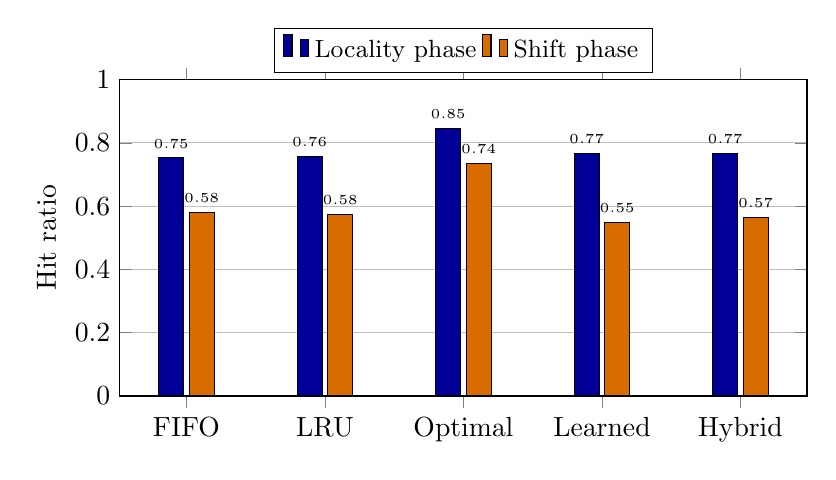
\begin{tikzpicture}
\begin{axis}[ybar,width=0.85\textwidth,height=5.6cm,bar width=9pt,ymin=0,ymax=1,
 ylabel={Hit ratio},symbolic x coords={FIFO,LRU,Optimal,Learned,Hybrid},xtick=data,
 legend style={at={(0.5,1.02)},anchor=south,legend columns=2,font=\small},ymajorgrids,enlarge x limits=0.12,
 nodes near coords,every node near coord/.append style={font=\tiny,/pgf/number format/fixed,/pgf/number format/precision=2}]
\addplot[fill=blue!60!black] coordinates {(FIFO,0.7525)(LRU,0.7575)(Optimal,0.845)(Learned,0.7675)(Hybrid,0.7675)};
\addplot[fill=orange!85!black] coordinates {(FIFO,0.58)(LRU,0.575)(Optimal,0.735)(Learned,0.5475)(Hybrid,0.565)};
\legend{Locality phase,Shift phase}
\end{axis}
\end{tikzpicture}
\caption{Hit ratio of each policy before and after the shift (seed 307).}
\label{fig:hit}
\end{figure}

\begin{figure}[H]
\centering
\begin{tikzpicture}
\begin{axis}[width=0.88\textwidth,height=5.6cm,xlabel={Reference index},ylabel={Rolling hit ratio},ymin=0.3,ymax=1,xmin=50,xmax=800,
 legend style={at={(0.5,1.02)},anchor=south,legend columns=4,font=\small},ymajorgrids]
\addplot[blue!70!black,thick] table[col sep=comma,x=t,y=LRU]{../results/rolling_hit.csv};
\addplot[red!80!black,thick] table[col sep=comma,x=t,y=Learned]{../results/rolling_hit.csv};
\addplot[green!50!black,thick] table[col sep=comma,x=t,y=Hybrid]{../results/rolling_hit.csv};
\addplot[black!60,thick] table[col sep=comma,x=t,y=Optimal]{../results/rolling_hit.csv};
\draw[dashed] (axis cs:400,0.3) -- (axis cs:400,1);
\legend{LRU,Learned,Hybrid,Optimal}
\end{axis}
\end{tikzpicture}
\caption{Rolling hit ratio (window of 50 references). The dashed line marks the workload shift.}
\label{fig:roll}
\end{figure}

\section{Analysis of the Workload Shift}
\textbf{All policies get worse.} In the shift phase the active set is the whole 10-page space while only 4 frames exist, and references are far less predictable. Every policy loses hit ratio, even Optimal (84.5\% $\to$ 73.5\%). That 11-point drop is the unavoidable part: it comes from the workload being harder, not from a poor policy.

\textbf{Which policy degrades most?} On the main trace the Learned policy drops most (22.0 points), then Hybrid (20.3), LRU (18.3), FIFO (17.3) and Optimal (11.0) (Table~\ref{tab:main}). However, the 20-trace study shows this ordering is \emph{not} reliable: Learned, LRU and Hybrid all lose about 20 points ($20.3\pm3.2$, $20.4\pm2.5$, $21.1\pm2.6$), well within one standard deviation of each other (Table~\ref{tab:multi}). The honest conclusion is that the online policies degrade by roughly the same amount, and all of them degrade about 7--9 points more than Optimal. FIFO's smaller drop mostly reflects that it starts lower.

\textbf{What the tree learned.} The tree (\texttt{results/learned\_tree.txt}) splits first on page id: pages 6--9 are marked almost certain to be evicted, and the remaining decisions use frequency and age. In the locality phase this is a good shortcut, since cold pages are rarely needed again. This helps on the main trace (76.8\% vs.\ 75.8\% for LRU) but not on average (74.3\% vs.\ 74.5\%), so with 4 frames and this trace the tree offers at most a small and unreliable gain over LRU. In the browsing phase pages 5--9 are as likely as pages 0--4, so ``evict the high page ids'' is probably the wrong rule, and accumulated frequency counts go stale. This likely explains why Learned ends slightly below LRU in the shift phase (54.1\% vs.\ 54.2\% on average, 54.8\% vs.\ 57.5\% on the main trace), although I did not run an ablation to confirm the cause.

\textbf{Effect of the hybrid guard.} Hybrid recovers a little on the main trace (56.5\% vs.\ 54.8\%) but gives no measurable benefit over 20 traces (54.0\% vs.\ 54.1\%). The 40-reference window reacts slowly and the shadow LRU is itself not much better than the tree here, so there is little to gain from falling back to it (Figure~\ref{fig:roll}).

\textbf{Limitations.} The traces are synthetic and tiny (4 frames, 10 pages), the tree is intentionally small and trained once, and the guard window was not tuned. A larger memory, a real trace, online retraining, or removing the page-id feature could change the picture~\cite{lykouris2018}.

\section{Conclusion}
FIFO, LRU and Optimal give understandable baselines and an upper bound. A small decision tree trained on locality behaviour slightly matches or beats LRU on one trace but gives no reliable gain on average, and it is no more robust than LRU when the workload shifts. All online policies lose about 18--21 points of hit ratio after the shift, versus 12 for Optimal. The main lesson is that a learned OS component must be validated across many traces and under workload change before it is trusted over a simple classical heuristic.

\section*{Reproducibility and AI Disclosure}
Run \texttt{./run.sh} (or \texttt{python3 src/run\_experiment.py}) from the repository root; it regenerates all files in \texttt{results/}. The report is built with \texttt{pdflatex term\_paper.tex} in \texttt{report/}. An AI assistant (Claude) helped with the implementation and drafting. I reviewed the code, results and analysis and can explain each part.

\begin{thebibliography}{9}\small
\bibitem{belady1966} L.~A. Belady, ``A study of replacement algorithms for a virtual-storage computer,'' \emph{IBM Systems Journal}, vol.~5, no.~2, pp.~78--101, 1966.
\bibitem{denning1968} P.~J. Denning, ``The working set model for program behavior,'' \emph{Communications of the ACM}, vol.~11, no.~5, pp.~323--333, 1968.
\bibitem{silberschatz} A.~Silberschatz, P.~B. Galvin and G.~Gagne, \emph{Operating System Concepts}, 10th ed., Wiley, 2018 (Ch.~10, Virtual Memory).
\bibitem{cart} L.~Breiman, J.~Friedman, R.~Olshen and C.~Stone, \emph{Classification and Regression Trees}, Wadsworth, 1984.
\bibitem{lykouris2018} T.~Lykouris and S.~Vassilvitskii, ``Competitive caching with machine learned advice,'' in \emph{Proc. 35th International Conference on Machine Learning (ICML)}, 2018, pp.~3296--3305.
\end{thebibliography}
\end{document}
